
\section*{Introduction}

Seasonal influenza virus infects 5--15\% of the global population every year causing an estimated 250,000 to 500,000 deaths annually \cite{flufactsheet}.
Vaccination remains the most effective public health response available.
However, frequent viral mutation results in viruses that escape previously acquired human immunity.
The World Health Organization (WHO) selects vaccine viruses to match circulating viruses, but because the process of vaccine development and distribution requires several months to complete, accurate vaccine strain selection requires a prediction of which viruses will predominate approximately one year after vaccine viruses are selected.
Current vaccine predictions favor viruses that are distinct from prior vaccine viruses in the hemagglutinin (HA) protein, which acts as the primary target of human immunity.
The hemagglutination inhibition (HI) assay \cite{hirst1943studies} is used to measure the degree of cross-reactivity between pairs of circulating viruses.
HI assays are fundamental for vaccine strain selection, but they are laborious and low-throughput compared to genome sequencing \cite{Wood:2012ii}.
As a result, researchers have developed computational methods to predict influenza fitness from sequence data alone \cite{Luksza:2014hj,Steinbruck:2014kq,Neher:2014eu}.

Despite the promise of these sequence-only models, they explicitly omit experimental measurements of antigenic or functional phenotypes.
Recent developments in computational methods and influenza virology have made it feasible to integrate these important metrics of influenza fitness into a single predictive model.
For example, phenotypic measurements of antigenic drift are now accessible through phylogenetic models \cite{Neher:2016hy} and functional phenotypes for HA are available from deep mutational scanning experiments \cite{Lee2018}.
We describe an approach to integrate previously disparate sequence-only models of influenza evolution with high-quality experimental measurements of antigenic drift and functional constraint.

The influenza community has long recognized the importance of incorporating HI phenotypes and other experimental measurements of viral phenotypes with existing forecasting methods into an extensible, open source framework that can be used by professional virologists in their vaccine design process \cite{Gandon:2016gz,Morris:2017ea,Lassig:2017hr}.
Although several distinct efforts have made progress in using HI phenotypes to evaluate the evolution of seasonal influenza \cite{Steinbruck:2014kq,Neher:2016hy}, these methods stop short of developing a complete forecasting framework wherein the evolutionary contribution of HI phenotypes can be compared and contrasted with new and existing fitness metrics.
Here, we provide the first such open source long-term forecasting framework for seasonal influenza.
With this framework, we show that HI phenotypes enable more accurate long-term forecasts of A/H3N2 populations compared to previous metrics based on epitope mutations alone.
However, we also find that phylogenetic fitness metrics based on recent growth of circulating clades consistently outperform any combination of genotypic or phenotypic metrics, suggesting that existing mechanistic models of seasonal influenza evolution are missing critical components.

\section*{Results}

\subsection*{A distance-based model of seasonal influenza evolution}

\begin{figure*}[t]
  \begin{center}
  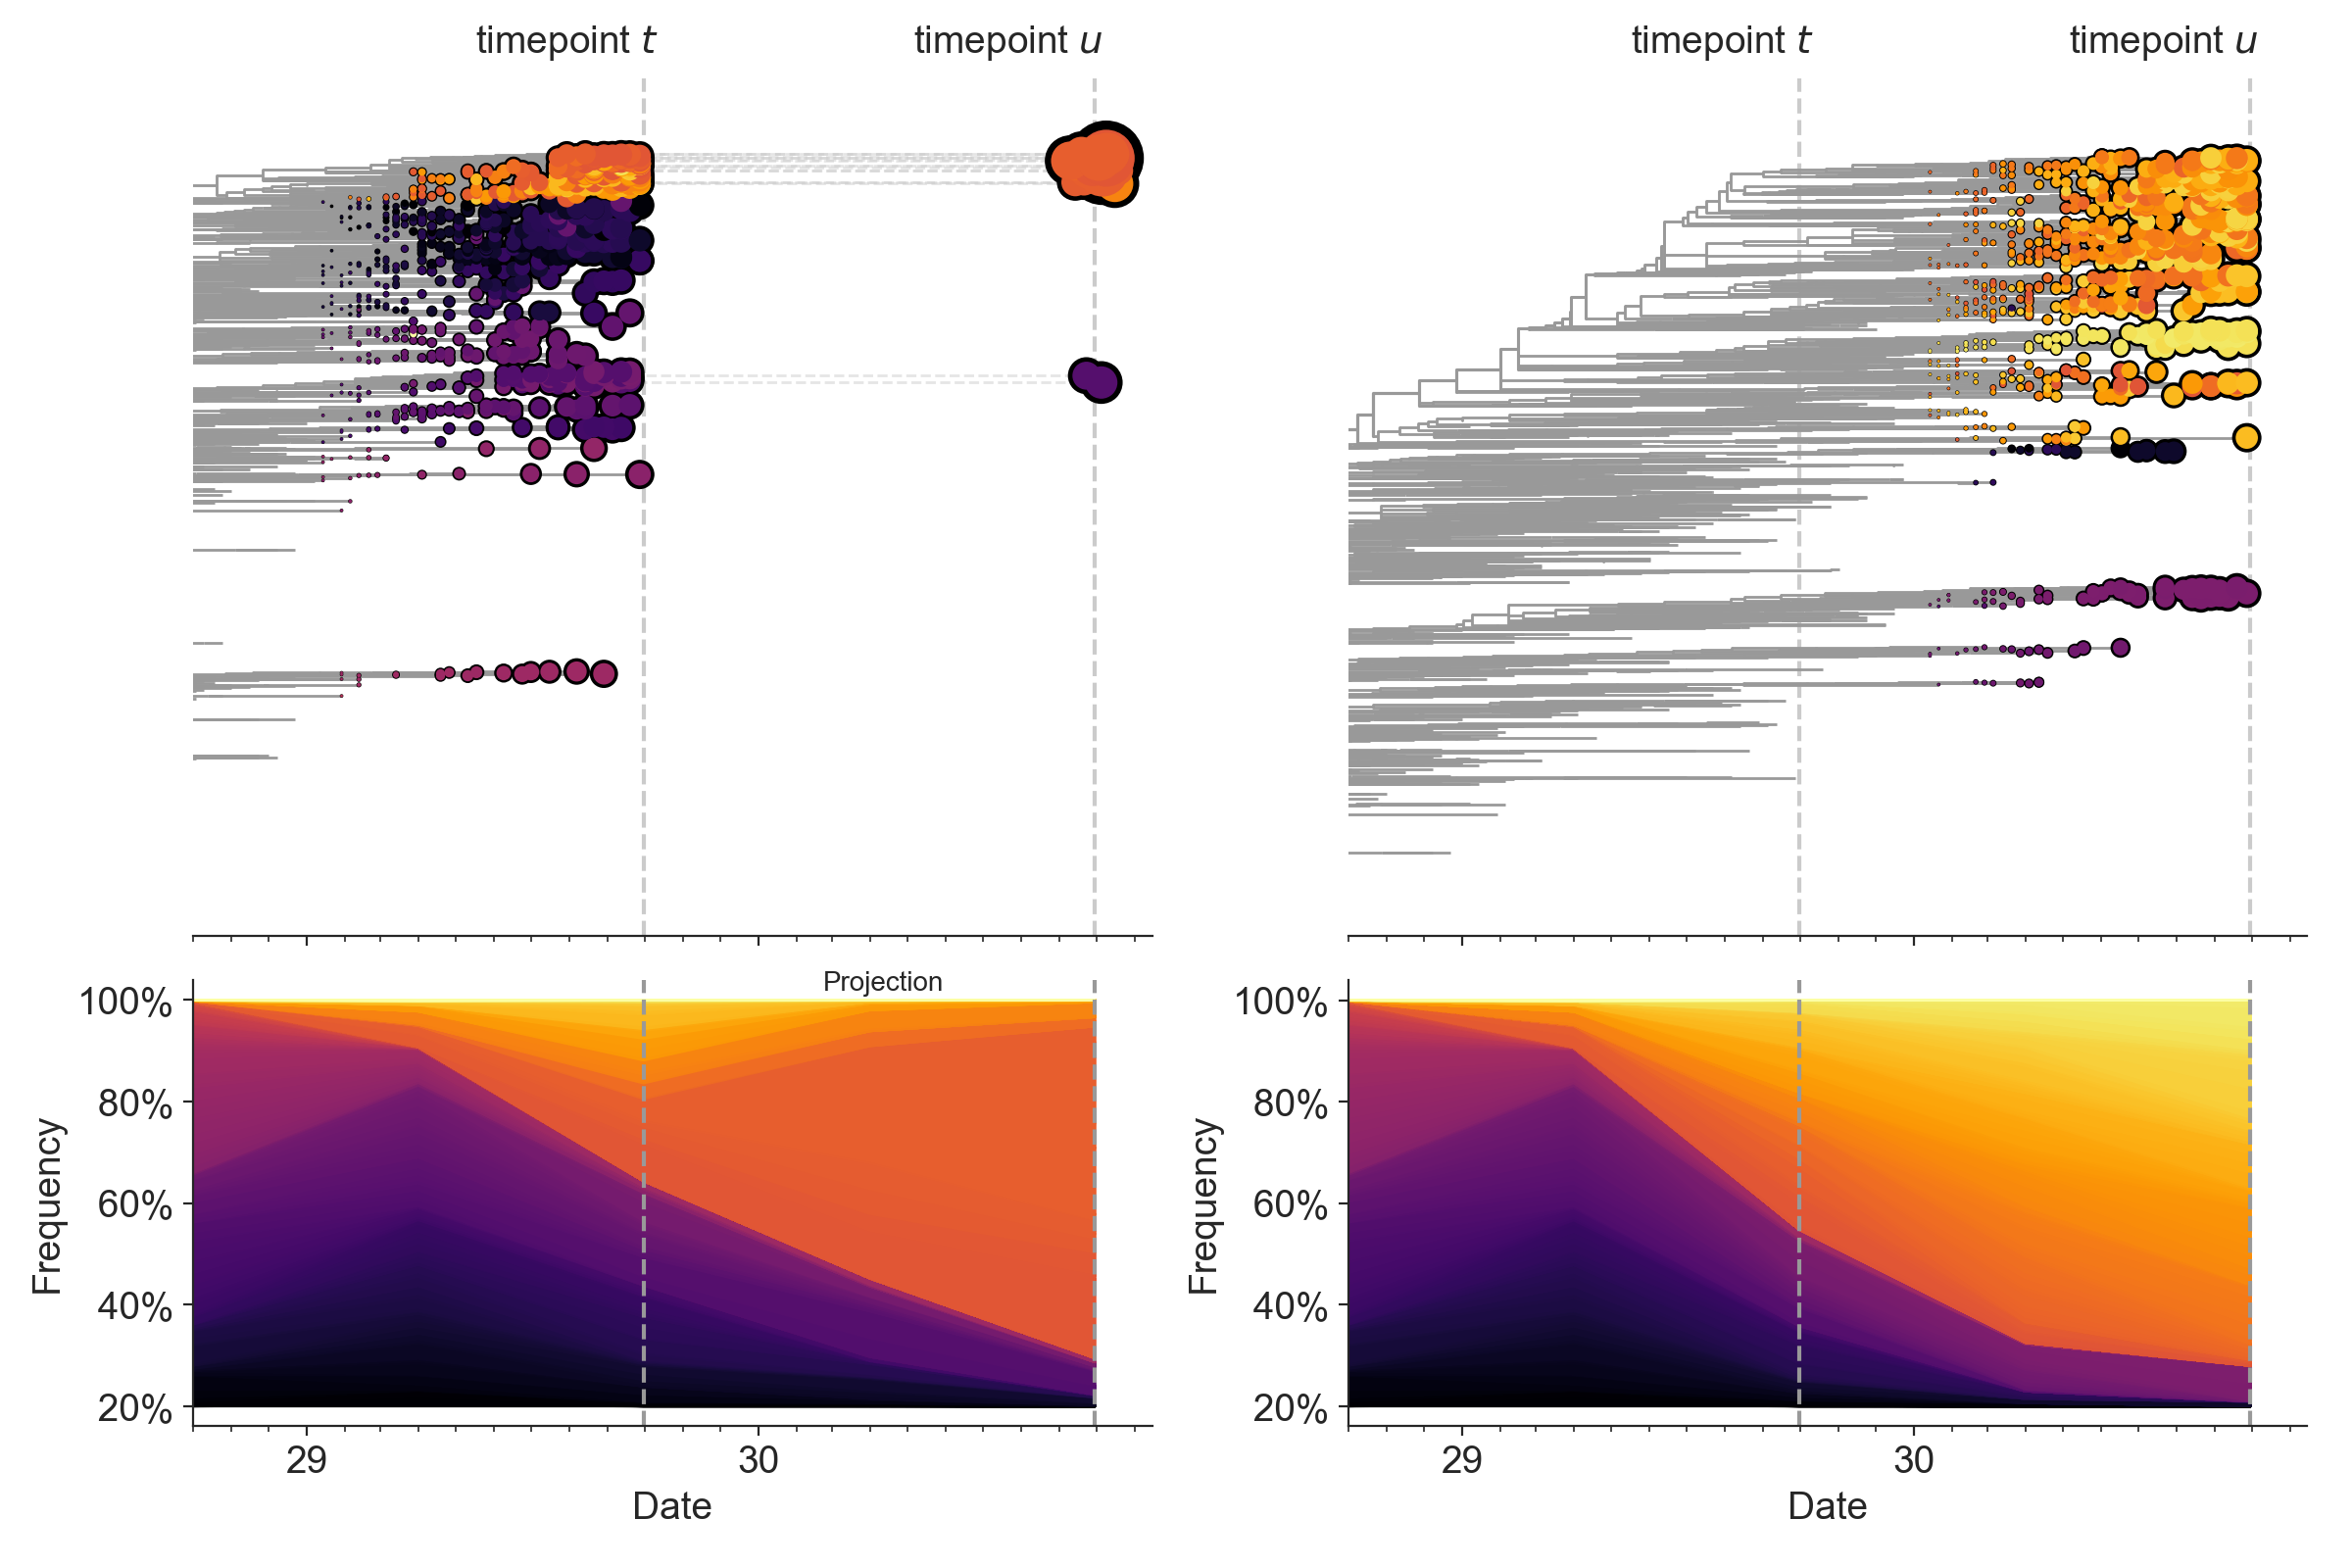
\includegraphics[width=\columnwidth]{figures/distance-based-fitness-model.png}
  \caption{
    Schematic representation of the fitness model wherein the fitness of samples at timepoint $t$ is used to minimize the distance between projected samples from that timepoint and the observed population at timepoint $u$ one year in the future.
    A) A phylogeny at timepoint $u=$April 2004 shows the observed population at that timepoint.
    The vertical dashed line delineates the previous timepoint of $t=$April 2003 where the size and color of each sample indicates the projected frequency of those samples one year in the future based on the composite model of delta frequency, HI cross-immunity, and non-epitope mutations.
    Bright yellow samples indicate those with the highest projected frequency and closest to the observed future population one year in the future.
    B) The density of average distances between samples at different timepoints show how the model estimates the future population from the current population.
    The blue line indicates the distance between populations at timepoints $t$ and $u$, or the best estimate by a naive model that projects no change in sample frequencies.
    The orange line shows the distance between the observed future population at timepoint $u$ and the estimated population at that time ($\hat{u}$) produced by projecting the frequency of samples at timepoint $t$ based on estimates of sample fitness.
    The green line shows the distance between the observed future population and itself.
    Notably, the estimated future population shifts the distribution of the naive model closer to zero.
  }
  \label{fig:model}
  \end{center}
\end{figure*}

Here, we present a model of seasonal influenza evolution inspired by the exponential growth model of \cite{Luksza:2014hj}.
As with this original model, we seek to forecast the frequencies of viral populations one year in advance by applying an exponential growth factor to each virus sample scaled by an estimate of the sample's fitness (Fig.~\ref{fig:model}).
We estimate the frequency of virus samples every six months using a smoothed KDE kernel to represent the frequency of each sample.
We estimate viral fitness with biologically-informed metrics including those originally defined by \cite{Luksza:2014hj} of epitope cross-immunity and non-epitope mutations as well as four more recent metrics including hemagglutination inhibition (HI) cross-immunity \cite{Neher:2016hy}, deep mutational scanning (DMS) mutational effects \cite{Lee2018}, local branching index (LBI) \cite{Neher:2014eu}, and change in clade frequency over time (delta frequency).
We fit models by learning coefficients for each fitness metric either individually or in linear combinations from training data and select the best of these models using time-series cross-validation.
After selecting optimal models from training and validation, we evaluate the true out-of-sample errors of these models on additional data that were held out from the initial model fitting and tuning.
Importantly, our models find fitness coefficients that minimize the normalized average Hamming distance between the observed population one year in the future and the estimated population produced by the exponential growth model.
With this approach, we avoid the intrinsic variability of ancestral sequence reconstruction associated with previous clade-based models.
However, we retain the benefits of fitting models to highly similar samples found within clades and enable future forecasting efforts for pathogens whose sequences are not amenable to standard phylogenetic inference.

\subsection*{Models accurately forecast evolution of simulated populations of {A/H3N2-like viruses}}

The long-term evolution of influenza A/H3N2 hemagglutinin has been previously described as a balance between positive selection for substitutions at epitopes that enable escape from adaptive immunity and purifying selection on domains required to maintain the protein's primary functions of binding and membrane fusion \cite{Bush:1999vj,Neher2013,Luksza:2014hj,Koelle:2015dh}.
To test the ability of our models to accurately detect these evolutionary patterns under controlled conditions, we simulated the long-term evolution of A/H3N2-like viruses under purifying and positive selection for 30 years (Methods).
These selective constraints produced phylogenetic structures and accumulation of epitope and non-epitope mutations that were consistent with phylogenies of natural A/H3N2 HA (Supplemental Figure \ref{sup_fig:simulated_h3n2_ha_phylogeny}).
We fit models to these simulated populations using all sequence-only fitness metrics.

We hypothesized that fitness metrics associated with viral success such as epitope cross-immunity, LBI, and delta frequency would be assigned positive coefficients, while the non-epitope mutations metric would be assigned a negative coefficient.
We reasoned that both LBI and delta frequency would individually outperform the mechanistic metrics as both of these growth metrics estimate recent clade success regardless of the mechanistic basis for that success.
Correspondingly, we expected that a combined model of epitope cross-immunity and non-epitope mutations would perform as well as or better than the growth metrics.
In addition to these four estimates of viral fitness, we tested models based on both the true fitness of each sample as measured by the simulator and a naive model under which the exponential growth factor is set to one and populations do not change composition over the one year forecasting period.
The distances estimated under the naive model represent the average distance between the current and future timepoints.

\begin{figure*}[t]
  \begin{center}
  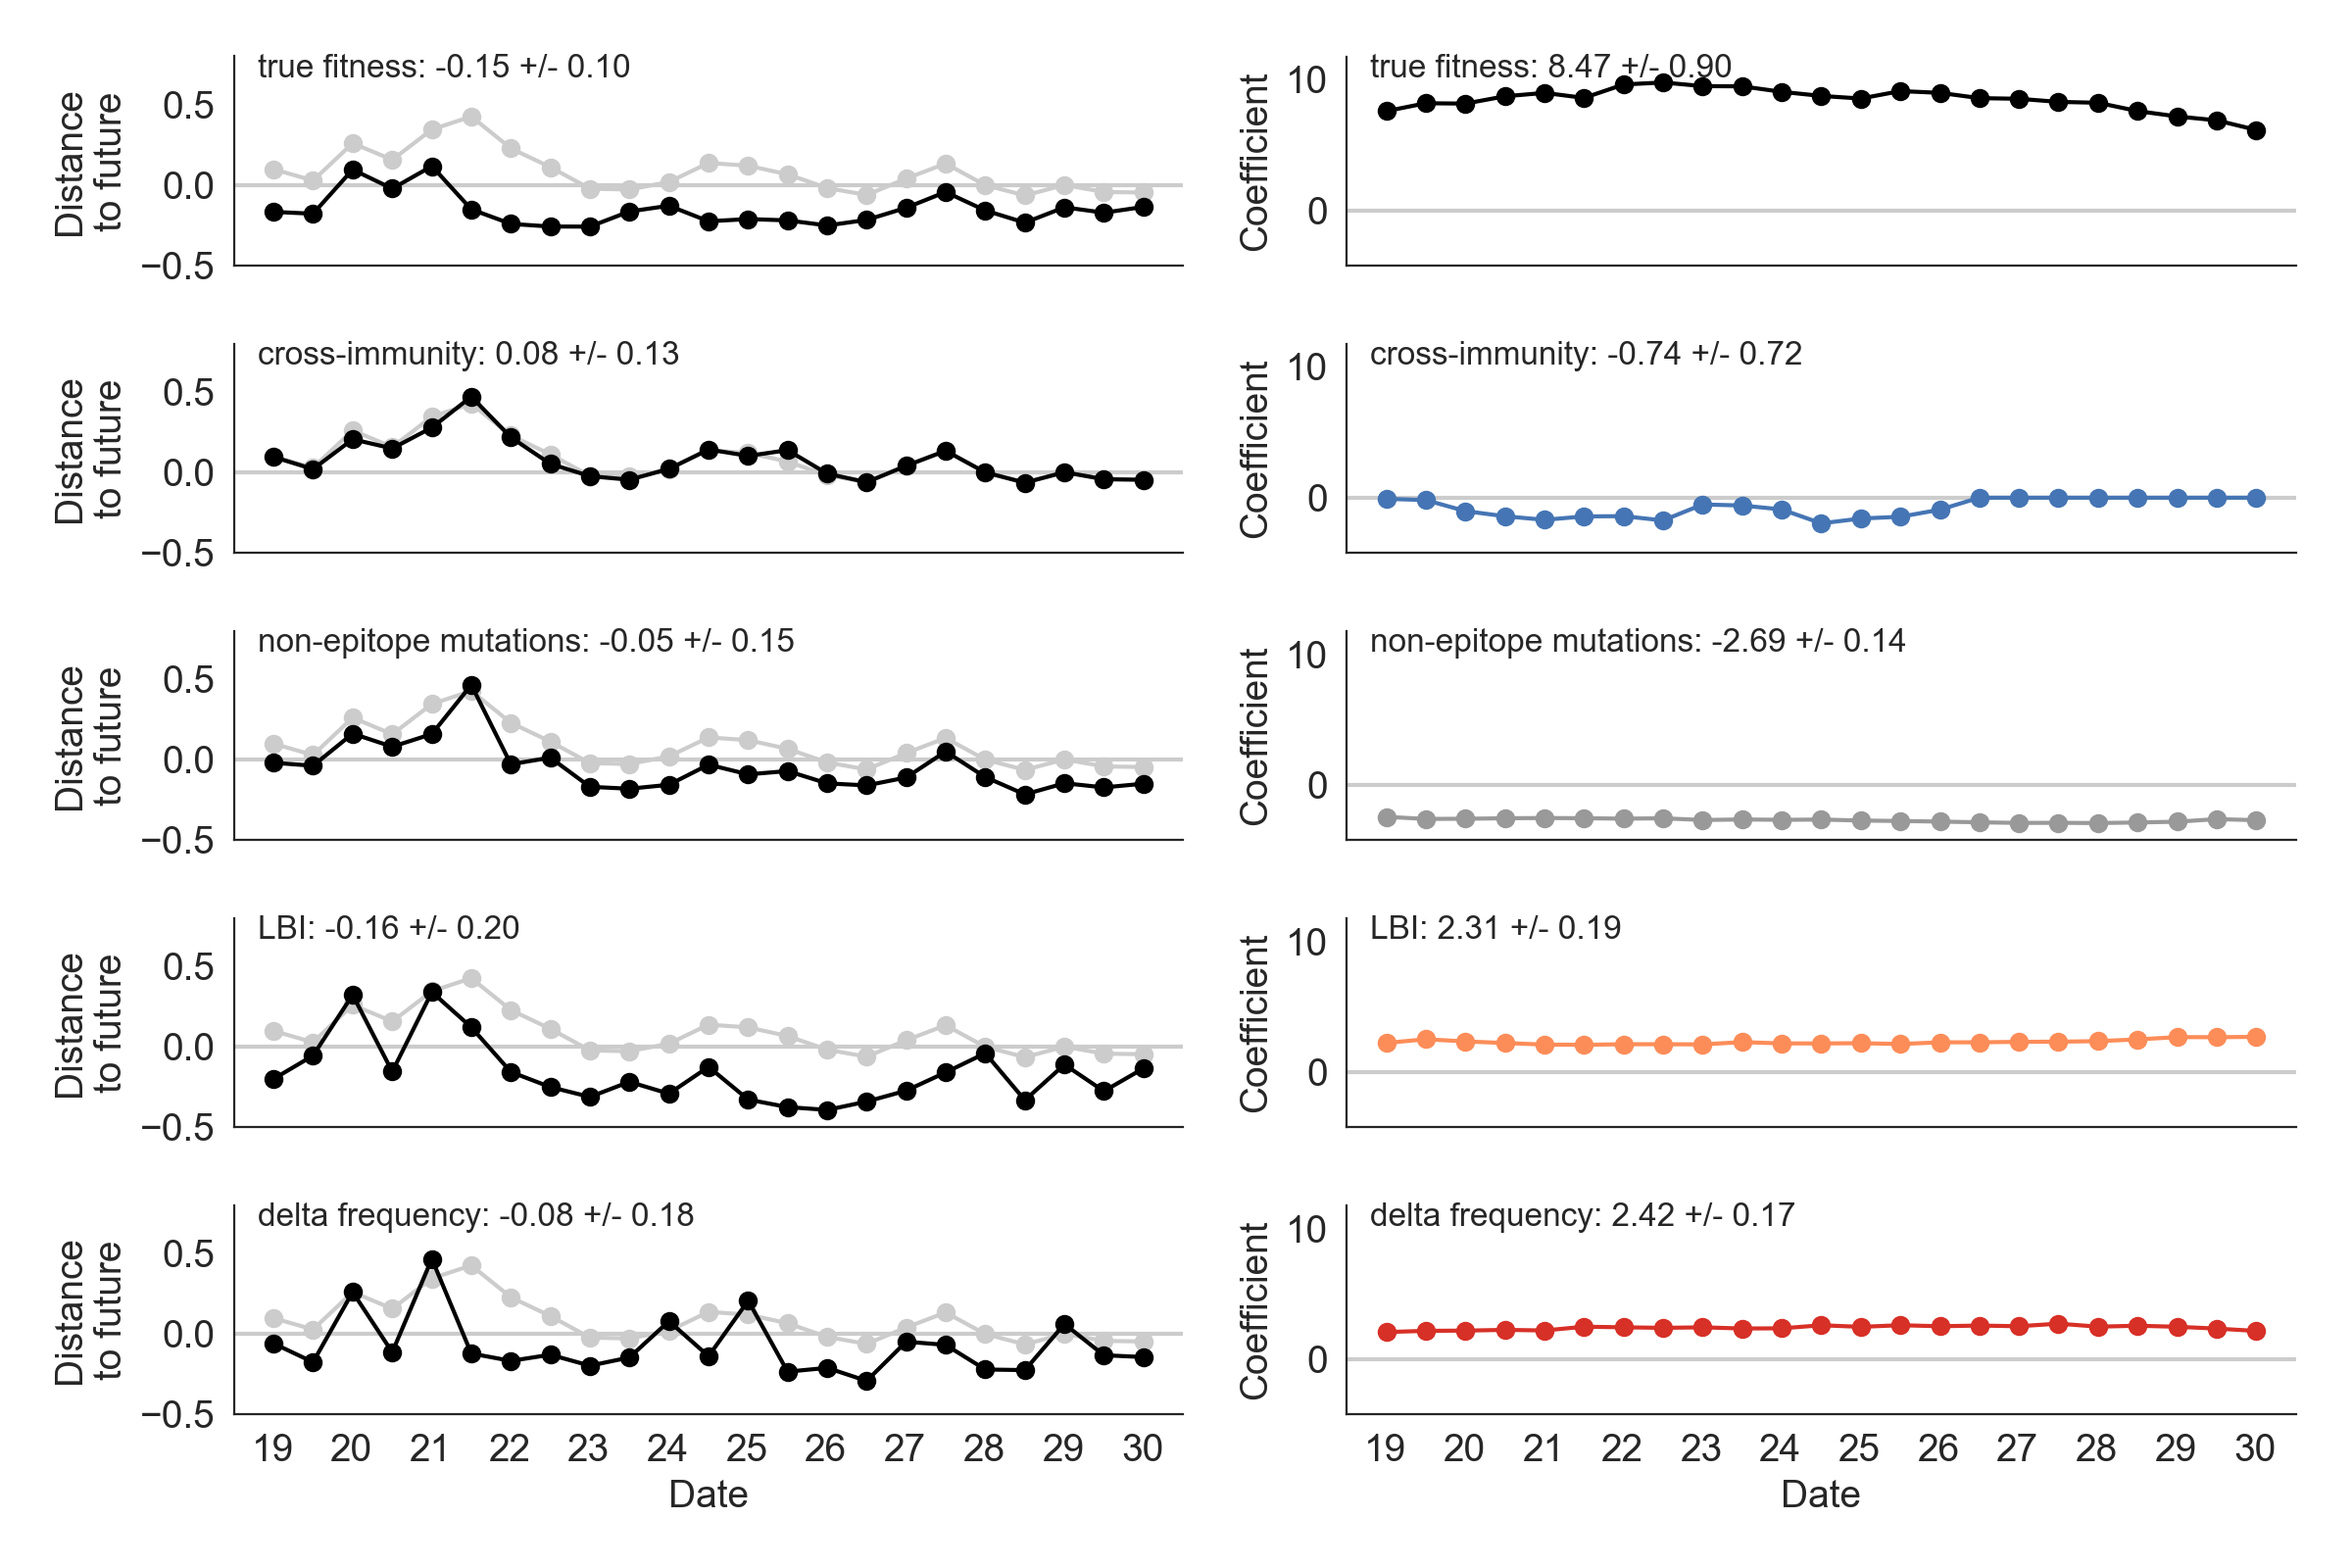
\includegraphics[width=\textwidth]{figures/unadjusted-model-accuracy-and-coefficients-for-simulated-populations.png}
  \caption{Model a) coefficients and b) accuracy for simulated populations of A/H3N2-like viruses.}
  \label{fig:unadjusted_model_accuracy_and_coefficients_for_simulated_populations}
  \end{center}
\end{figure*}

As expected, the true fitness model was the most consistently accurate, estimating distances to the future less than or equal to zero at 21 of 23 (91\%) timepoints (Fig.~\ref{fig:unadjusted_model_accuracy_and_coefficients_for_simulated_populations}).
The naive model was the least accurate with an average estimated distance of 0.07 +/- 0.10 (Supplemental Fig.~\ref{sup_fig:distance_of_simulated_populations_between_timepoints}).
The non-epitope mutations metric received a consistently negative coefficient and also outperformed the naive model with an average distance less than zero.
LBI and delta frequency both received positive coefficients and outperformed the mechanistic metrics on average.
LBI performed as well as the true fitness predictor, on average, but suffered from higher variability in distance estimates.
Surprisingly, epitope cross-immunity performed no better than the naive model and received a negative average coefficient, despite the anticipated benefit of epitope mutations that could escape exposure-dependent fitness penalties.
Similarly, the combined model of epitope cross-immunity and non-epitope mutations did not perform better than the individual non-epitope mutations model (Supplemental Fig.~\ref{sup_fig:unadjusted_composite_model_accuracy_and_coefficients_for_simulated_populations}).
From these results, we concluded that our method can accurately estimate the evolution of simulated populations, but that the fitness of samples under our simulated conditions was dominated by purifying selection rather than by positive selection at epitope sites.

To determine which evolutionary constraints the LBI model represented, we fit an additional composite models including LBI and both mutation metrics.
We expected the coefficients from these composite models to reveal which individual metrics were mutually exclusive or beneficial.
For example, if LBI accounted for antigenic drift, the coefficients for LBI and epitope cross-immunity should exhibit negatively correlated changes through time.
Interestingly, we found that this composite model nearly converged to a LBI-only model with small or zero-valued coefficients for both mutation metrics in the last half of the simulated timepoints (Supplemental Fig.~\ref{sup_fig:unadjusted_composite_model_accuracy_and_coefficients_for_simulated_populations}).
These results indicate that LBI alone can account for the predictive contributions of both cross-immunity and non-epitope mutations.
In contrast, when we fit a composite model of delta frequency, cross-immunity, and non-epitope mutations, both delta frequency and non-epitope mutations maintained their respective positive and negative coefficients across all timepoints.
This result suggests that LBI and delta frequency measure qualitatively different components of fitness despite both being similar growth metrics.

\subsection*{Model accuracy and coefficients reflect historical patterns of A/H3N2 evolution}

Next, we trained and validated models for individual fitness predictors using 23 years of natural A/H3N2 populations spanning from October 1992 to October 2015.
We held out samples collected between October 2015 and April 2019 for model testing.
In addition to the sequence-only models we tested on simulated populations, we also fit models for our new fitness metrics based on experimental phenotypes from HI and DMS assays.
We hypothesized that both HI and DMS phenotype metrics would be assigned positive coefficients, as they estimate increased antigenic drift and beneficial mutations, respectively.
As antigenic drift is generally considered to be the primary evolutionary pressure on natural A/H3N2 populations \cite{Smith:2004jc,Bedford:2014bf,Luksza:2014hj}, we expected that epitope cross-immunity and HI phenotypes would be individually more predictive than non-epitope mutations or DMS phenotypes.
Previous research \cite{Neher:2016hy} and our simulation results also led us to expect that LBI and delta frequency would outperform other individual mechanistic metrics.

\begin{figure*}[t]
  \begin{center}
  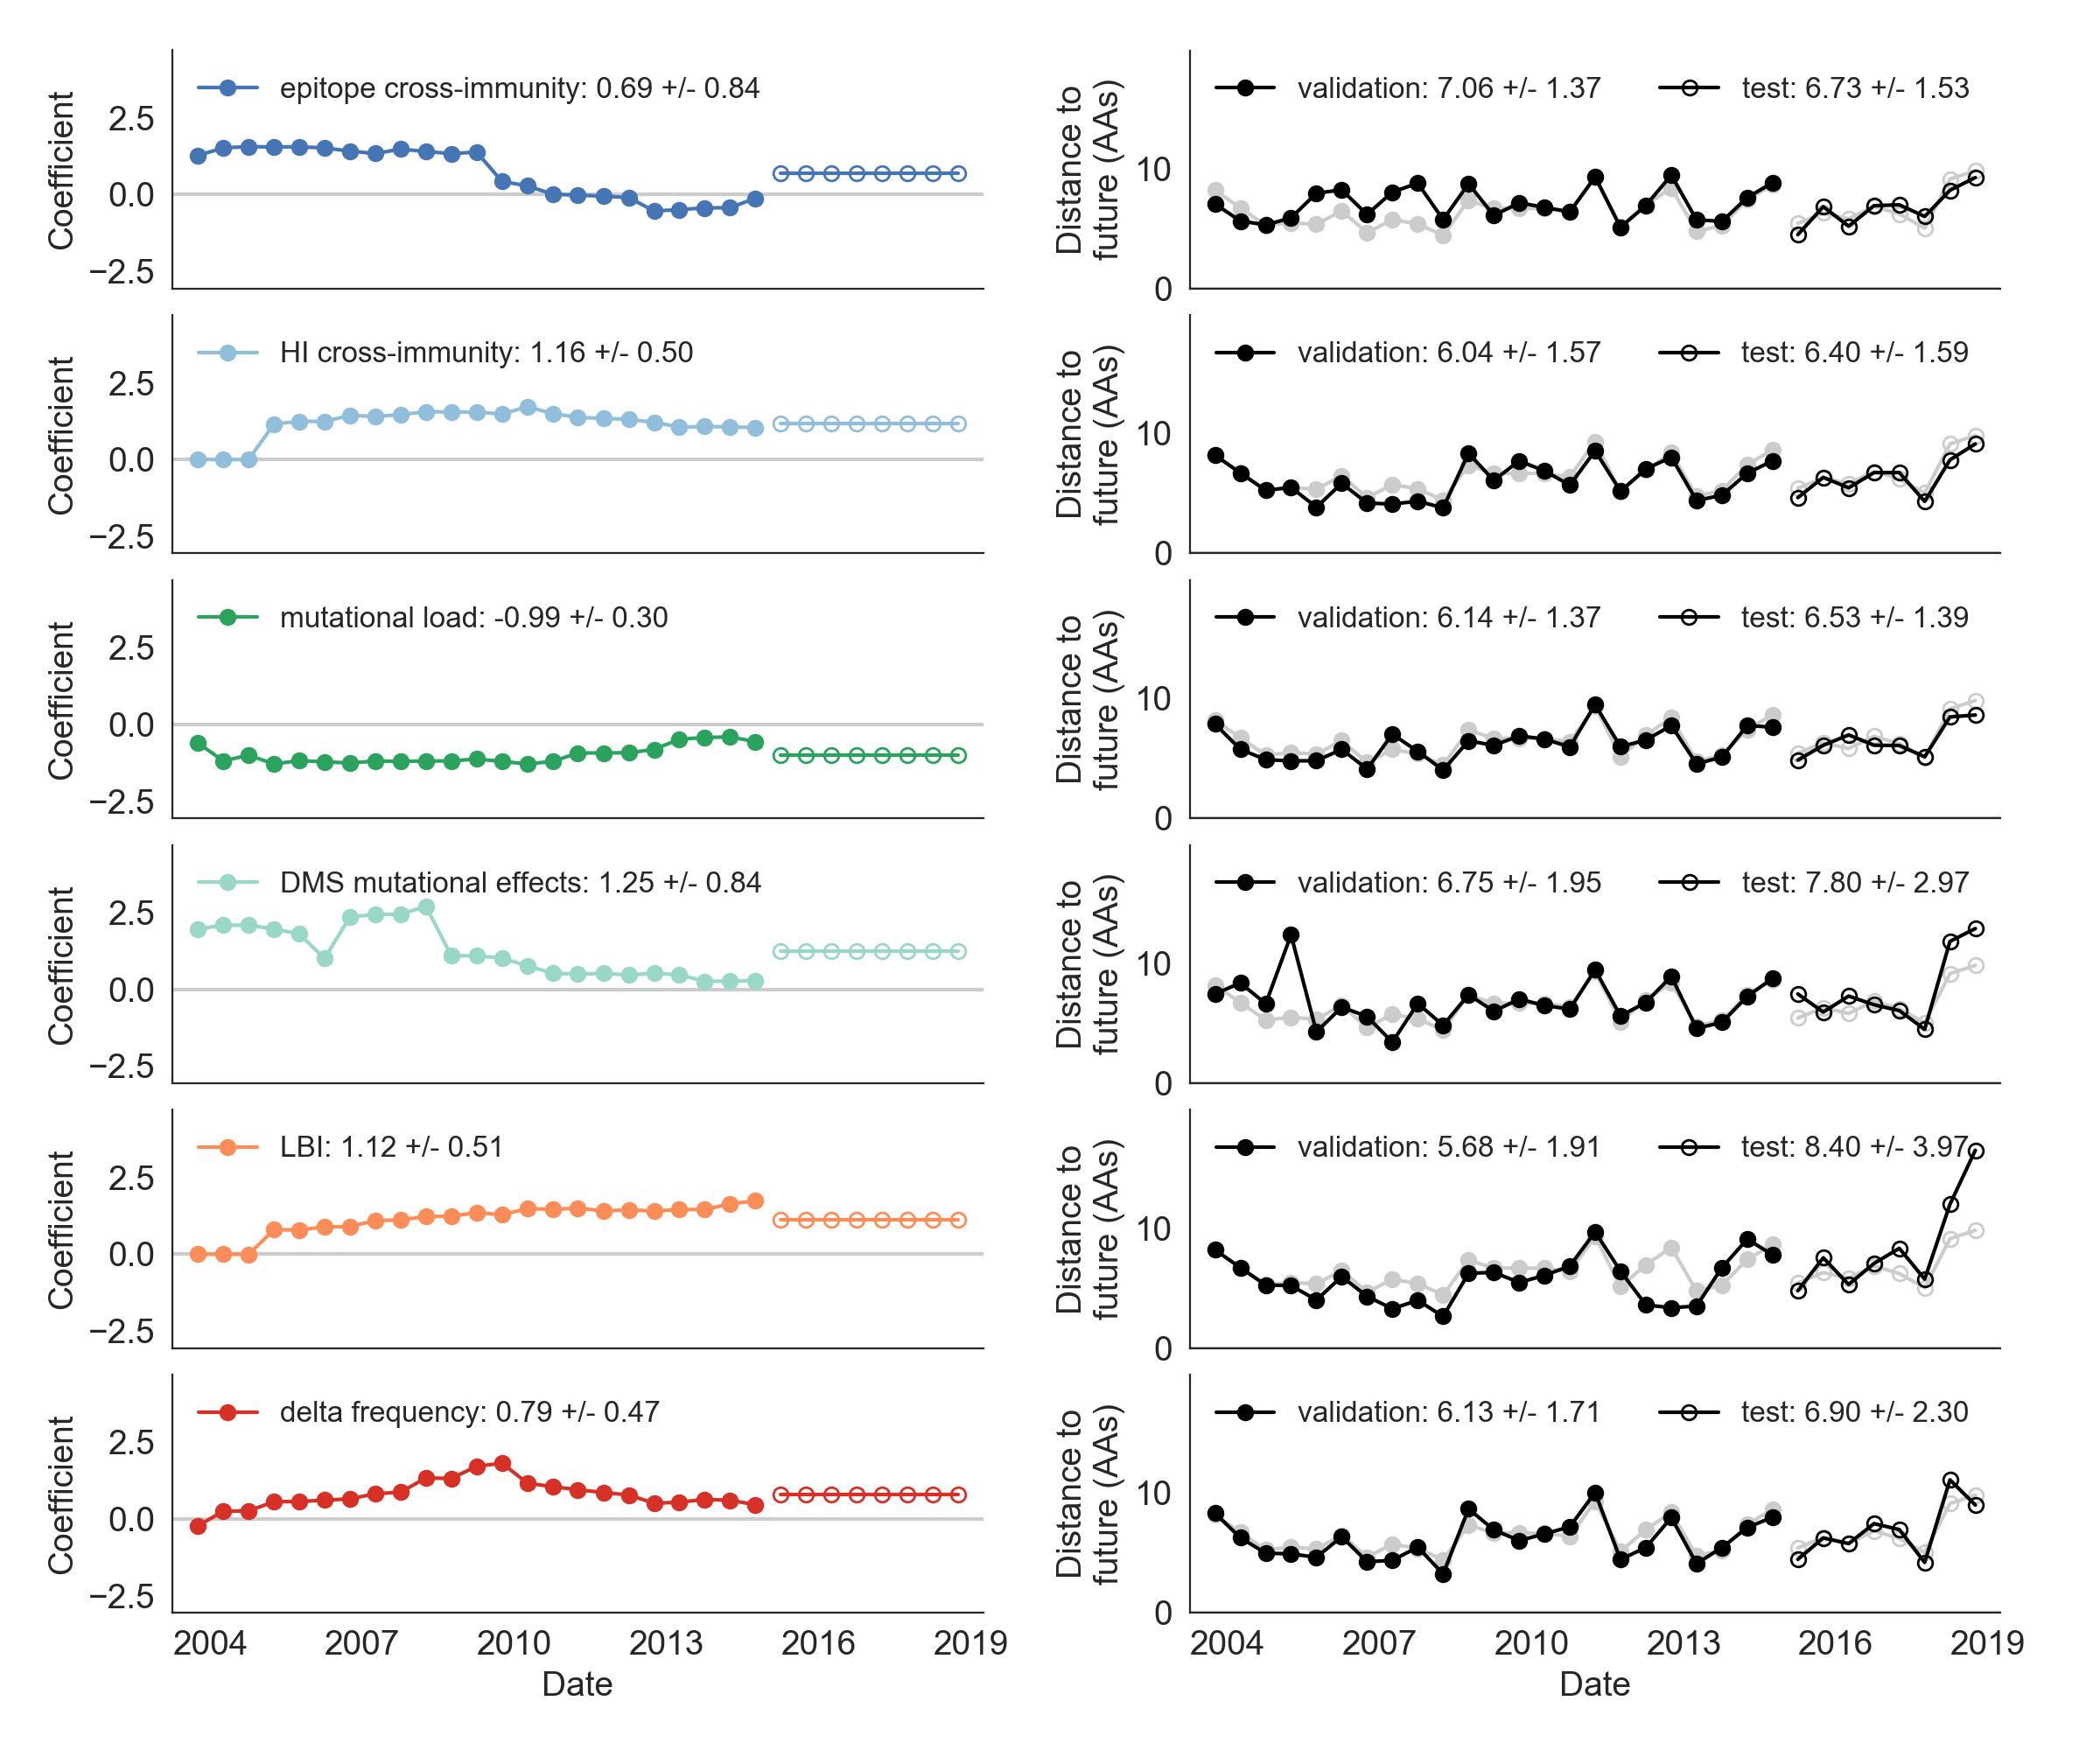
\includegraphics[width=\textwidth]{figures/unadjusted-model-accuracy-and-coefficients-for-natural-populations.png}
  \caption{Model a) coefficients and b) accuracy for natural populations of A/H3N2 viruses.}
  \label{fig:unadjusted_model_accuracy_and_coefficients_for_natural_populations}
  \end{center}
\end{figure*}

The average distance per year between natural populations was 0.21 +/- 0.16, indicating that the diversity of natural populations was three times that of simulated populations (Supplemental Fig.~\ref{sup_fig:distance_of_natural_populations_between_timepoints}).
Biologically-informed metrics generally performed better than the naive model for natural populations with the exceptions of the epitope cross-immunity and DMS phenotypes metrics (Fig.~\ref{fig:unadjusted_model_accuracy_and_coefficients_for_natural_populations}).
Surprisingly, neither antigenic fitness metric outperformed the best functional constraint metric of non-epitope mutations.
Indeed, epitope cross-immunity only outperformed the naive model at 11 of 29 timepoints (34\%), while HI phenotypes outperformed the naive model at 24 timepoints (83\%).
Epitope cross-immunity was also the only metric whose coefficient started at a positive value and transitioned to a negative value through the validation period.
This change in coefficient and the greater accuracy of epitope mutations in the earliest timepoints suggested that positive selection may have weakened at these epitope sites over time.
In contrast, HI phenotypes maintained a positive coefficient across most timepoints and consistently outperformed the epitope model.
The HI phenotypes metric may benefit from being able to constantly update its antigenic model at each timepoint with recent experimental phenotypes, while the epitope cross-immunity metric is forced to give a constant weight to the same 49 sites throughout time.

Non-epitope mutations also outperformed the DMS phenotypes metric with an average distance to the future of 0.11 +/- 0.16 compared to 0.21 +/- 0.19.
In contrast to \cite{Luksza:2014hj}, where the coefficient of the non-epitope mutations metric was hardcoded to -0.5, our model learned a consistently stronger coefficient of -2.03 +/- 0.33.
Notably, the DMS metric performed slightly better for timepoints before April 2010 and performed no better than the naive model thereafter.
This result is consistent with the DMS model overfitting to the evolutionary history of the background strain used to perform the DMS experiments, A/Perth/16/2009.
Alternate implementations of less background-dependent DMS metrics never performed better than the non-epitope mutations metric (Supplemental Fig.~\ref{sup_fig:unadjusted_DMS_model_accuracy_and_coefficients_for_natural_populations}).
These results suggest that any mutation at a non-epitope site is deleterious for globally circulating strains, despite the more fine-grained fitness constraints of within-host infections.

LBI was the best individual fitness metric and the only metric to estimate an average distance to the future that was less than zero (Fig.~\ref{fig:unadjusted_model_accuracy_and_coefficients_for_natural_populations}).
Delta frequency performed as well as HI cross-immunity and non-epitope mutations.
While delta frequency should, in principle, measure the same aspect of viral fitness as LBI, these results clearly show that the current implementations of these metrics represent qualitatively different fitness components.
Both of these phylogenetic growth metrics strongly depend on a sufficient density of samples, as revealed by the weaker model coefficients for these metrics in the earliest validation timepoints when there are relatively few samples.

\subsection*{Composite models outperform models with individual fitness metrics}

The results suggested that combinations of the best individual metrics like LBI, delta frequency, non-epitope mutations, and HI phenotypes could produce even more accurate models.
To this end, we fit models for X combinations of these metrics and evaluated their distance to the future and coefficients relative to the corresponding individual metrics.
We found results (Supplemental Fig.~\ref{sup_fig:unadjusted_composite_model_accuracy_and_coefficients_for_natural_populations}).

\subsection*{Models enable selection of vaccine candidate strains}

\subsection*{Forecasts predict the rise of A1b/131K and A1b/135K sub-clades in September 2020}

See Fig.~\ref{fig:nextstrain_forecasts}.

\begin{figure*}[t]
  \begin{center}
  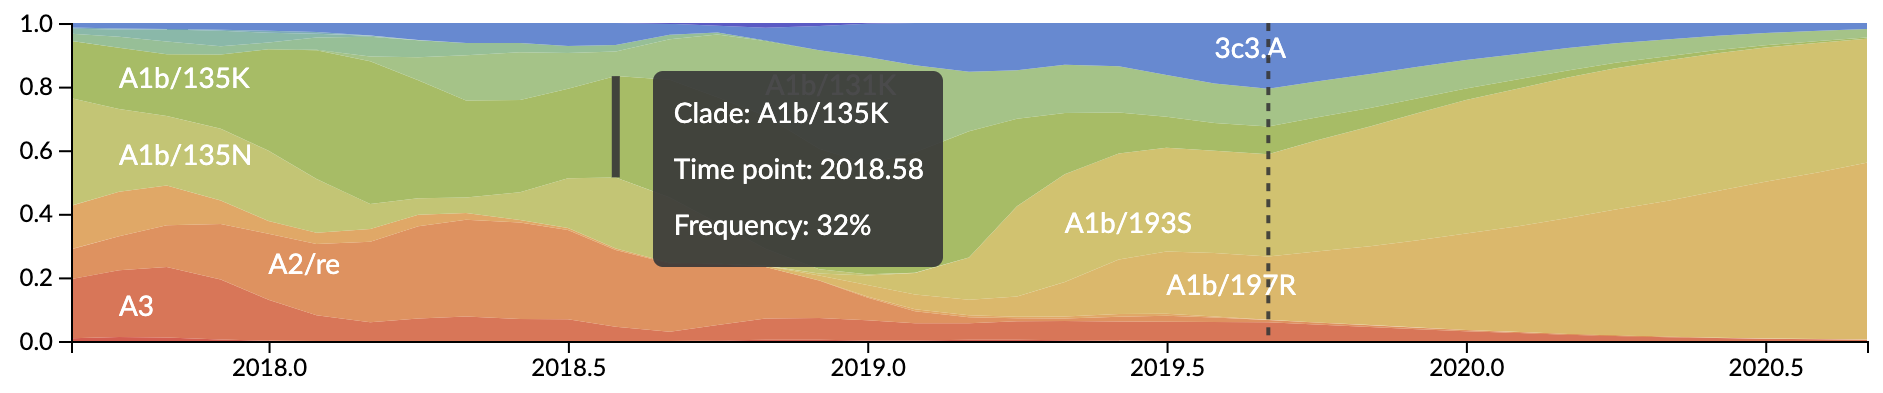
\includegraphics[width=\textwidth]{figures/nextstrain-forecasts-for-september-2020.png}
  \caption{Live forecasts on nextstrain.org from our best model for September 2020.}
  \label{fig:nextstrain_forecasts}
  \end{center}
\end{figure*}

\section*{Discussion}

Discussion.

\section*{Methods}

\subsection*{Simulation of influenza A/H3N2-like populations}

We simulated the long-term evolution of A/H3N2-like viruses with SANTA-SIM \cite{Jariani2019} for 40 years where 100 generations was equivalent to 1 year.
We discarded the first 10 years as a burn-in period, selected the next 20 years for model fitting and validation, and held out the last 10 years as out-of-sample data for model testing.
Each simulated population was seeded with the full length HA from A/Beijing/32/1992 (NCBI accession: U26830.1) such that all simulated sequences contained signal peptide, HA1, and HA2 domains.
We defined purifying selection across all three domains, allowing the preferred amino acid at each site to change at a fixed rate over time.
We additionally defined exposure-dependent selection for 49 putative epitope sites in HA1 \cite{Luksza:2014hj} to impose an effect of cross-immunity that would allow mutations at those sites to increase viral fitness despite underlying purifying selection.
We modified the SANTA-SIM source code to enable the inclusion of true fitness values for each sample in the FASTA header of the sampled sequences from each generation.
This modified implementation is available at https://github.com/huddlej/santa-sim/tree/emit-fitness.

\subsection*{Strain selection for natural populations}

For model training and validation, we selected XX HA sequences of length >=1,700 nucleotides that were sampled between October 1994 and October 2015.
To account for known variation in sequence availability by region, we subsampled the selected sequences to a representative set of 10 viruses per month with even sampling across 10 global regions including Africa, Europe, North America, China, South Asia, Japan and Korea, Oceania, South America, Southeast Asia, and West Asia.
We excluded all samples with ambiguous year, month, and day annotations and prioritized samples with more available HI titer measurements.

For model testing, we extended the set of training and validation sequences to include HA sequences that were sampled between October 2015 and April 2019.
We used these test sequences to evaluate the out-of-sample error of fixed model parameters learned during training and validation.

\subsection*{Phylogenetic interference}

For each timepoint in model training, validation, and testing, we selected the subsampled HA sequences with collection dates up to that timepoint.
We aligned sequences with the augur align command \cite{Hadfield2018} and MAFFT v7.407 \cite{Katoh2002}.
We inferred initial phylogenies for HA sequences at each timepoint with IQ-TREE v1.6.10 \cite{Nguyen2014}.
To reconstruct time-resolved phylogenies, we applied TreeTime v0.5.6 \cite{Sagulenko2018} with the augur refine command.

\subsection*{Frequency estimation}

To account for uncertainty in collection date and sampling error, we applied a kernel density estimation (KDE) approach to calculate global sample frequencies.
Specifically, we constructed a Gaussian kernel for each sample with the mean at the reported collection date and a variance of one month, roughly corresponding to the average lag time between sample collection and submission to the GISAID database.
We estimated the frequency of each sample at each timepoint by calculating the cumulative density function of each KDE between the current and previous timepoint and normalizing the resulting values to sum to one.
We implemented this logic in the augur frequencies command.

\subsection*{Model fitting and evaluation}

\subsubsection*{Fitness model}

As in \cite{Luksza:2014hj}, we assumed that influenza A/H3N2 populations can be described by an exponential growth model.
Under this model, we estimated the future frequency of the global population, $\hat{X}$, at some time in the future, $t + \Delta{t}$, based on the current frequency, $x_{i}(t)$, and fitness, $f_{i}(t)$, of each sample $i$ as follows where the resulting future frequencies were normalized to one by $\frac{1}{Z(t)}$.

$$
\hat{X}(t + \Delta{t}) = \frac{1}{Z(t)}\sum_{i}x_{i}(t)\exp(f_{i}(t))
$$

We defined the fitness of each sample at time $t$ as the additive combination of one or more fitness metrics, $f_{i,m}$, scaled by fitness coefficients, $\beta_{m}$.

\subsubsection*{Model target}

For a model based on any given combination of fitness metrics, we found the fitness coefficients that minimized the mean weighted Hamming distance between the estimated and observed future populations at time $u = t + \Delta{t}$ as defined by,

$$
\Delta(X(u), \hat{X}(u)) = \frac{\sum_{i}\sum_{j}x_{i}(t)\exp(f_{i}(t)\Delta{t})x_{j}(u)d_{i,j} - \sum_{j}\sum_{k}x_{j}(u)x_{k}(u)d_{j,k}}{\sum_{i}\sum_{j}x_{i}(t)x_{j}(u)d_{i,j}}.
$$

The first term in the numerator measures the mean distance between estimated and observed future populations, the second term measures the average distance of the future population to itself, and the denominator measures the average distance between the current and future populations.
When a model accurately estimates the average distance of the future population to itself, the metric evaluates to zero.
When the estimated sequence diversity is closer to the center of the future population's observed diversity, the metric evaluates to a negative proportion.
We applied the Nelder-Mead minimization algorithm as implemented in SciPy \cite{SciPy} to learn fitness coefficients that minimize the average of this distance metric over all timepoints in a given training window.

\subsubsection*{Time-series cross-validation}

To obtain unbiased estimates for the out-of-sample errors of our models, we adopted the standard cross-validation strategy of training, validation, and testing.
We divided our available data into an initial training and validation set spanning October 1994 to October 2015 and an additional testing set spanning October 2015 to April 2019.
We partitioned our training and validation data into six month seasons corresponding to winter in the Northern Hemisphere (October--April) and the Southern Hemisphere (April--October) and trained models to estimate frequencies of populations one year into the future from each season in six-year sliding windows.
To calculate validation error for each training window, we applied the resulting model coefficients to estimate the future frequencies for the year after the last timepoint in the training window.
These validation errors informed our tuning of hyperparameters including a L1 regularization of the fitness coefficients, the LBI neighborhood parameter $\tau$, and the length of the training window itself.
Finally, we fixed the coefficients for each model at the mean values across all training windows and applied these fixed models to the test data to estimate the true forecasting accuracy of each model on previously unobserved data.

\subsection*{Fitness metrics}

\subsubsection*{Antigenic drift}

\subsubsection*{Functional constraint}

\subsubsection*{Clade growth}
